\subsubsection{Data}

The data of the exercise is reported here.
\begin{itemize}
	\item 10 sensors
	\item $T_{transmission} = 10 \text{ minutes}$
	\item $b = 2000 \text{ bit}$
	\item $E_b = 5 \text{ mJ}$
	\item $E_c = 50 \text{ nJ/bit}$
	\item $E_{tx}(d) = k \cdot d^2 \text{ nJ/bit}$
	\item $k = 1 \text{ nJ/bit/$m^2$}$
\end{itemize}

The sensors of the parking lot have fixed positions, reported in the following table.
\begin{table}[H]
\centering 
\begin{tabular}{| c | c |}
	\hline 
	\rowcolor{bluepoli!40}
	\textbf{Sensor} & \textbf{Position}\T\B \\
	\hline 
	1 & (1, 2) \T\B\\
	2 &(10, 3) \T\B\\
	3 & (4, 8) \T\B\\
	4 & (15, 7) \T\B\\
	5  & (6, 1) \T\B\\
	6  & (9, 12) \T\B\\
	7  & (14, 4) \T\B\\
	8  & (3, 10) \T\B\\
	9  & (7, 7) \T\B\\
	10  & (12, 14) \T\B\\
	\hline
\end{tabular}
\\[10pt]
\caption{Sensor position table}
\label{table:sensor_position_table}
\end{table}

The following picture describes the distributions of sensors.
\begin{figure}[H]
    \centering
    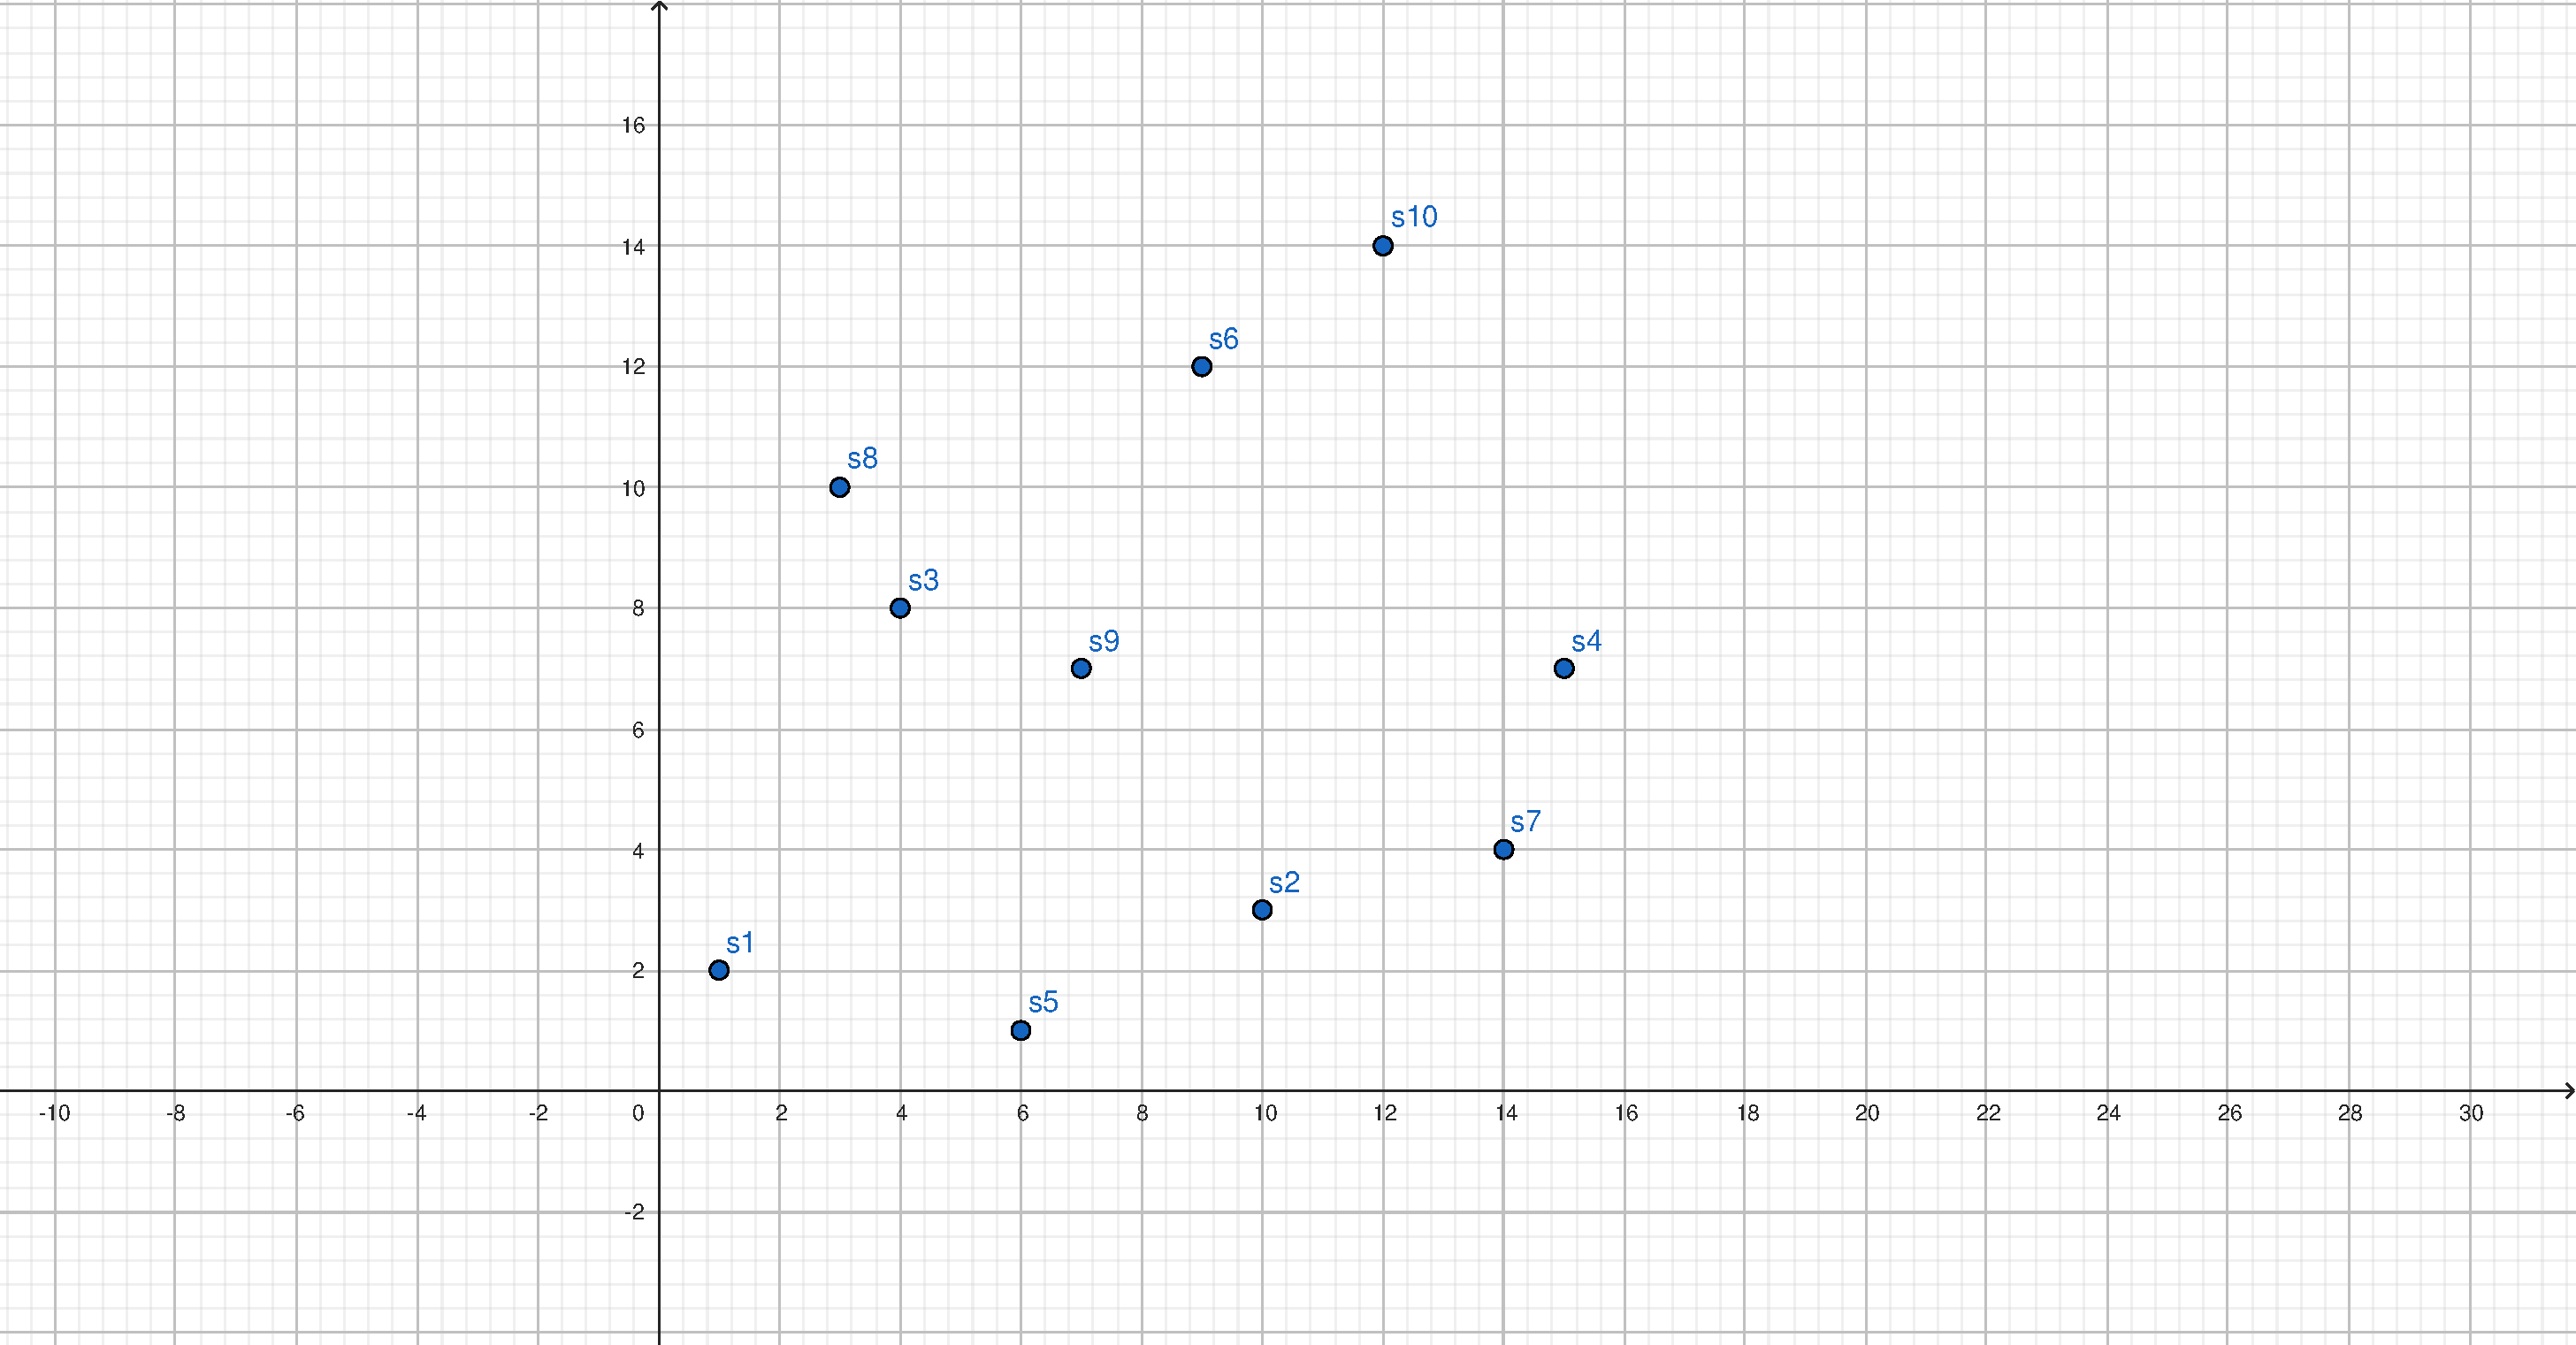
\includegraphics[width=\linewidth, height=0.3\textheight, keepaspectratio]{points.pdf}
    \caption{Sensor distribution}
    \label{fig:Sensor_distribution}
\end{figure}


\subsubsection{Lifetime of the system with sink in (20,20)}
In order to compute the lifetime of the system when the sink position is ($x_s, y_s$) = (20, 20), we need to compute the lifetime of the furthest sensor from the sink.\\
We calculated the distance of every sensor from the sink, the values are reported in the following table.

\begin{table}[H]
\centering 
\begin{tabular}{| c | c | c |}
	\hline 
	\rowcolor{bluepoli!40}
	\textbf{Sensor} & \textbf{Position} & \textbf{Distance from sink}\T\B \\
	\hline 
	1 & (1, 2) & $\sqrt{685} \text{ m}$ \T\B\\
	2 &(10, 3) & $\sqrt{389} \text{ m}$ \T\B\\
	3 & (4, 8) & 20 m\T\B\\
	4 & (15, 7) & $\sqrt{194} \text{ m}$ \T\B\\
	5  & (6, 1) & $\sqrt{557} \text{ m}$ \T\B\\
	6  & (9, 12) & $\sqrt{185} \text{ m}$ \T\B\\
	7  & (14, 4) & $2\sqrt{73} \text{ m}$ \T\B\\
	8  & (3, 10) & $\sqrt{389} \text{ m}$ \T\B\\
	9  & (7, 7) & $13\sqrt{2} \text{ m}$ \T\B\\
	10  & (12, 14) & 10 m\T\B\\
	\hline
\end{tabular}
\\[10pt]
\caption{Distances from sink}
\end{table}

The distance between the sink and the furthest sensor, sensor 1, is: 
\[ 
distance_1 = d \{(1, 2) , (20, 20)\} = \sqrt{(20-1)^2 + (20-2)^2} = \sqrt{685} m 
\]
We compute the energy consumed by sensor 1 as:
\[
E_{cycle, 1} = E_c \cdot b + E_{tx, 1}(d) \cdot b = 50 nJ/bit \cdot 2000 \text{ bit} + 1 nJ/bit/m^2 \cdot 685 m^2 \cdot 2000 \text{ bit} = 1.47 mJ
\]
The lifetime, measured in number of cycles, is:
\[
L_{cycles} = E_b / E_{cycle, 1} = 3.401 \text{ cycles}
\]
Assuming that each sensor transmits at the beginning of the ten minutes, the system will last for three cycles and during the fourth cycle the furthest sensor will die.

\subsubsection{Optimal sink position}
In order to maximize the system's lifetime, we need to maximize the lifetime of the sensor node that consumes the most energy. The energy consumption for a transmission is given by:
\[
E_{cycle} = E_c \cdot b + E_{tx}(d) \cdot b = E_c \cdot b + k \cdot d^2 \cdot b
\]
Since the energy for the circuitry, $E_c$, is constant, the energy consumption grows with the distance. In order to maximize the lifetime of the system, we need to minimize the maximum distance between the sink and the furthest node. This problem is equivalent to that of finding the smallest circle enclosing all point on the cartesian plane, representing the positions of nodes.\\
A very efficient algorithm that can be used to solve the smallest enclosing circle problem is Welzl's algorithm, which finds a solution in O(n) time. 
The algorithm is recursive and uses two sets:
\begin{itemize}
	\item P: contains all input points;
	\item R: initially empty, at the end, contains point on the boundary of the minimum enclosing circle;
\end{itemize}
The base cases are the ones in which the smallest circle encloses three or less points:
\begin{itemize}
	\item if it doesn't enclose any point, the circle is undefined;
	\item if it encloses one point, the degenerate circle is the point itself and has radius zero;
	\item if it encloses two points or three points, there is just one circle passing through them;
\end{itemize}
At each step, select a point p from P and find the smallest enclosing circle of the other points:
\begin{itemize}
	\item  if p lies in D, D is the minimum enclosing circle;
	\item otherwise, p must be part of the boundary, remove p from P and add it to R, recurse on the next element of set P;
\end{itemize}
A Python implementation of the algorithm can be found below.

\begin{python}
import math
import random

# data structures
class Point:
    def __init__(self, x, y):
        self.x = x
        self.y = y

class Circle:
    def __init__(self, c, r):
        self.c = c
        self.r = r

# checks wheter point p is inside circle c 
def isInside(c, p):
    return math.dist([c.c.x, c.c.y], [p.x, p.y]) <= c.r

# checks if all points in ps are in c 
def isValidCircle(c, ps):
    return all(isInside(c, point) for point in ps)

# helper method to get a circle defined by 3 points
def getCircleCenter(bx, by, cx, cy):
    b = bx * bx + by * by
    c = cx * cx + cy * cy
    d = bx * cy - by * cx
    return Point((cy * b - by * c) / (2 * d), (bx * c - cx * b) / (2 * d))

# returns the circle passing for 2 points (a,b)
def circleFromTwo(a, b):
    c = Point((a.x + b.x) / 2.0, (a.y + b.y) / 2.0)
    return Circle(c, math.dist([a.x, a.y], [b.x, b.y]) / 2.0)

# returns the circle passing for 3 points (a,b,c)
def circleFromThree(a, b, c):
    i = getCircleCenter(b.x - a.x, b.y - a.y, c.x - a.x, c.y - a.y)
    i.x += a.x
    i.y += a.y
    return Circle(i, math.dist([i.x, i.y], [a.x, a.y]))

# minimum enclosing circle trivial cases
def minCircleTrivial(p):
    assert len(p) <= 3
    if not p:
        return Circle(Point(0, 0), 0)
    elif len(p) == 1:
        return Circle(p[0], 0)
    elif len(p) == 2:
        return circleFromTwo(p[0], p[1])

    for i in range(3):
        for j in range(i + 1, 3):
            c = circleFromTwo(p[i], p[j])
            if isValidCircle(c, p):
                return c
    return circleFromThree(p[0], p[1], p[2])

def welzl(p):
    pCopy = list(p)
    random.shuffle(pCopy)
    return welzlHelper(pCopy, [], len(pCopy))

def welzlHelper(p, r, n):
    if n == 0 or len(r) == 3:
        return minCircleTrivial(r[:])

    idx = random.randint(0, n - 1)
    pnt = p[idx]
    p[idx], p[n - 1] = p[n - 1], p[idx]

    d = welzlHelper(p, r, n - 1)

    if isInside(d, pnt):
        return d

    return welzlHelper(p, r + [pnt], n - 1)


# run algorithm on nodes positions
nodes_positions = [
    Point(1,2),
    Point(10,3),
    Point(4,8),
    Point(15,7),
    Point(6,1),
    Point(9,12),
    Point(14,4),
    Point(3,10),
    Point(7,7),
    Point(12,14)
]
mec = welzl(nodes_positions)

# print sink position
print("Sink position:", mec.c.x, mec.c.y)
print("Furthest node:", mec.r)
\end{python}

Running the algorithm, we get the following result:
\begin{verbatim}
Sink position: 6.871681415929204 7.65929203539823
Furthest node: 8.155012507169454
\end{verbatim}

Thus, the optimal position of the sink is approximately (6.87, 7.66) and the maximum distance from the sink to a node is of about 8.16 meters.\\
We can compute the lifetime of the system when the sink is in position (6.87, 7.66) as follows.

\[
E_{cycle, furthest} = E_c \cdot b + E_{tx, furthest}(d) \cdot b = 0.233 mJ
\]

\[
L_{cycles} = E_b / E_{cycle, furthest} = 21.443 \text{ cycles}
\]

Under the assumption that each sensor transmits at the beginning of the ten minutes, it will last 21 cycles and die in the next one.

\subsubsection{Tradeoff static and dynamic sink position}
